% ALGUNOS PAQUETES REQUERIDOS (EN UBUNTU): %
% ========================================
% %
% texlive-latex-base %
% texlive-latex-recommended %
% texlive-fonts-recommended %
% texlive-latex-extra %
% texlive-lang-spanish (en ubuntu 13.10) %
% ******************************************************** %

\documentclass[a4paper]{article}
\usepackage[utf8]{inputenc}
\usepackage{fancyhdr}
\usepackage[pdftex]{graphicx}
\usepackage{sidecap}
\usepackage{caption}
\usepackage{subcaption}
\usepackage{booktabs}
\usepackage{makeidx}
\usepackage{float}
\usepackage{array}
\usepackage{amsmath, amsthm, amssymb}
\usepackage{amsfonts}
\usepackage{sectsty}
\usepackage{wrapfig}
\usepackage{listings}
\usepackage{pgfplots}
\usepackage{enumitem}
\usepackage{hyperref}
\usepackage{listings}
\usepackage{listingsutf8}
\usepackage{pgfplotstable}
\usepackage{colortbl}
\usepackage{algpseudocode}
\usepackage[spanish,es-nodecimaldot]{babel}
\graphicspath{imagenes/}}

\linespread{factor}

\definecolor{mygreen}{rgb}{0,0.6,0}
\definecolor{mygray}{rgb}{0.5,0.5,0.5}
\pgfplotsset{compat=1.3}
\setlist[enumerate]{label*=\arabic*.}
\lstset{
	inputencoding=utf8/latin1,
	language=C++,
	basicstyle=\ttfamily,
	keywordstyle=\bfseries\color{blue},
	stringstyle=\color{red}\ttfamily,
	commentstyle=\color{mygreen}\ttfamily,
	morecomment=[l][\color{magenta}]{\#},
	numbers=left,
	numberstyle=\color{mygray}
}
\pgfplotstableset{% global config, for example in the preamble
  every head row/.style={before row=\toprule,after row=\midrule},
  every last row/.style={after row=\bottomrule},
  fixed,precision=2,
}

\usepackage{color} % para snipets de codigo coloreados
\usepackage{fancybox}  % para el sbox de los snipets de codigo

\definecolor{litegrey}{gray}{0.94}

% \newenvironment{sidebar}{%
% 	\begin{Sbox}\begin{minipage}{.85\textwidth}}%
% 	{\end{minipage}\end{Sbox}%
% 		\begin{center}\setlength{\fboxsep}{6pt}%
% 		\shadowbox{\TheSbox}\end{center}}
% \newenvironment{warning}{%
% 	\begin{Sbox}\begin{minipage}{.85\textwidth}\sffamily\lite\small\RaggedRight}%
% 	{\end{minipage}\end{Sbox}%
% 		\begin{center}\setlength{\fboxsep}{6pt}%
% 		\colorbox{litegrey}{\TheSbox}\end{center}}

\newenvironment{codesnippet}{%
	\begin{Sbox}\begin{minipage}{\textwidth}\sffamily\small}%
	{\end{minipage}\end{Sbox}%
		\begin{center}%
		\vspace{-0.4cm}\colorbox{litegrey}{\TheSbox}\end{center}\vspace{0.3cm}}



\usepackage{fancyhdr}
\pagestyle{fancy}
%\renewcommand{\chaptermark}[1]{\markboth{#1}{}}
\renewcommand{\sectionmark}[1]{\markright{\thesection\ - #1}}
\fancyhf{}
\fancyhead[LO]{Sección \rightmark} % \thesection\
\fancyfoot[LO]{\small{Nicolás Bukovits, Kevin Frachtenberg, Julián Len, Nicolás Len}}
\fancyfoot[RO]{\thepage}
\renewcommand{\headrulewidth}{0.5pt}
\renewcommand{\footrulewidth}{0.5pt}
%\setlength{\hoffset}{-0.8in}
\setlength{\textwidth}{16cm}
\setlength{\hoffset}{-1.1cm}
\setlength{\headsep}{0.5cm}
\setlength{\textheight}{25cm}
\setlength{\voffset}{-0.7in}
\setlength{\headwidth}{\textwidth}
\setlength{\headheight}{13.1pt}
\renewcommand{\baselinestretch}{1.1} % line spacing

\usepackage{caratula}

\newcommand{\ord}{\ensuremath{\operatorname{O}}}
\newcommand{\nat}{\ensuremath{\mathbb{N}}}

\begin{document}

\setcounter{page}{1}
\materia{Algoritmos y Estructuras de Datos III}
\submateria{Segundo Cuatrimestre de 2016}
\titulo{Trabajo Práctico III}
%\subtitulo{Grupo: }
\integrante{Nicolás Bukovits}{546/14}{nicobuk@gmail.com}
\integrante{Kevin Frachtenberg}{247/14}{kevinfra94@gmail.com}
\integrante{Julián Len}{467/14}{julianlen@gmail.com}
\integrante{Nicolás Len}{819/11}{nicolaslen@gmail.com}
\maketitle
% no footer on the first page
\thispagestyle{empty}

\newpage
\tableofcontents

\newpage
\section{Introducción}

Este trabajo es el resultado del estudio de una instancia del \textit{Traveling Salesman Problem}. El TSP (por sus siglas) es conocido en español como "Provlema del viajante", el cual sitúa a un viajero en búsqueda del camino más corto que cumpla ciertas condiciones las cuales, en general, son que debe recorrer distintas ciudades interconectadas sin pasar más de una vez por cada una. En nuestro caso de estudio, tenemos un jugador de \textit{Pokémon GO} en una ciudad en la que hay distintos puntos con 2 posibles características: los \textbf{gimnasios} y las \textbf{pokeparadas}. Los primeros son lugares que el jugador desea conquistar siendo que están, en un comienzo, bajo control del enemigo y para ello debe vencer a los pokemones enemigos utilizando los propios. Un pokemon es una criatura virtual que tiene un poder de ataque y de vida. Para vencer a los enemigos es necesaria una cierta cantidad de posiones, las cuales se obtienen de las pokeparadas. Cada una de ellas le otorga 3 posiones al jugador y la forma en que éste las guarda es en una mochila que tiene una capacidad máxima; si la mochila está llena y el jugador pasa por una pokeparada, las posiones son descartadas. Relacionando ambas ideas, estudiamos nuestra problemática considerando que las restricciones para hallar el camíno mínimo es que dados $n$ la cantidad de gimnasios, $m$ la cantidad de pokeparadas y $k$ el tamaño de la mochila, queremos pasar por todos los gimnasios siempre que tengamos la cantidad de posiones necesarias para capturarlo, que en ningún momento tengamos más posiones que $k$ y, obviamente, no pasar dos veces por el mismo lugar.

Para obtener la solución a este problema, se plantearon 4 formas distintas utilizando las técnicas algorítmicas vistas en la materia. Los mismos presentaron cada uno un desafío distinto, teniendo que aplicar métodos diferentes para resolverlos y cumplir con los requisitos exigidos.

Además de la resolución de los mismos, se procedió a demostrar la correctitud de
cada implementación. Esto fue acompañado a su vez de una justificación de la
complejidad temporal.

Cada ejercicio contó con su respectiva experimentación para corroborar que la
complejidad temporal teórica se cumpliera y en los casos donde el algoritmo
podía comportarse mejor, verlo reflejado de alguna manera.

Los experimentos contaron con diversas medidas para asegurar su efectividad de
las cuales las siguientes fueron iguales para los tres problemas:
\begin{itemize}
	\item{Sólo se midió el costo temporal de generar la solución, no
			de lectura y escritura del problema.}
	\item{Para la medición del tiempo se utilizó la biblioteca \texttt{chronos}
			con unidad de tiempo en microsegundos.}
\end{itemize}


En todos los casos, el input del programa se dió de la siguiente manera:
Una línea con tres valores enteros positivos, $n$, $m$ y $k$, separados por espacios; los valores $n$ y $m$ indican la cantidad gimnasios y paradas, respectivamente, mientras que $k$ indica el tamaño de la mochila. A continuación, siguen $n$ líneas, representando los gimnasios. Cada una contiene 3 enteros, $x$, $y$ y $p$, donde $x$ e $y$ indican la posición, y $p$ la cantidad de pociones necesarias para vencer el gimnasio. Las siguentes $m$ lineas indican la posición de las pokeparadas, cada una contiene dos enteros $x$ e $y$.

\newpage
\section{Ejercicio 1: Solución exacta}

  % \begin{figure}[ht]
  %   \begin{center}
  %     \includegraphics[width=0.5\columnwidth]{imagenes/pacman.png}
  %     \caption{Perdidos y con poca fuerza}
  %   \end{center}
  % \end{figure}

    % 1. Describir detalladamente el problema a resolver dando ejemplos del mismo y sus soluciones.
    \subsection{Descripción del problema y solución propuesta}
        En este primer acercamiento, se pidió realizar un algoritmo exacto que resuelva el problema en cuestión. El mísmo debía contener podas y estrategias que permitan mejorar el tiempo de ejecución pero que aseguren devolver la solución correcta (en caso de haber).

        Una solución existe cuando se pueden conquistar todos los gimnasios y además es exacta cuando se conquistan todos ellos recorriendo la menor distancia posible.

    % 2. Explicar de forma clara, sencilla, estructurada y concisa, las ideas desarrolladas para la resolución del problema. Utilizar pseudocódigo y lenguaje coloquial (no código fuente). Justificar por qué el procedimiento resuelve efectivamente el problema.
        Dado que nuestro problema es una instancia del TSP mencionado en la introducción, resolvimos encontrar la solución exacta utilizando la técnica de \textit{backtracking}. Esto es probar todas las soluciones posibles descartando la mayor cantidad que no sean correctas a la vez mediante el uso de \textit{podas}, para así obtener lo más rápido posible la solución correcta. Cada solución se  construye de manera tal que en cada iteración se agrega parte de una posible solución. En este caso, lo que se hace es recorrer el grafo desde cada nodo probando todos los caminos posibles, es decir, partiendo de cada gimnasio o pokeparada, conquistar todos los gimnasios pociones todas las formas posibles sin pasar dos veces por el mismo lugar. Las podas utilizadas fueron las siguientes:
            \begin{itemize}
                \item{Verificar al principio que dado pociones($g$) el número de pociones para un gimnasio $g$, \newline $\sum_{g \in Gimnasios} pociones(g) \leq m*3$ con $m$ cantidad de pokeparadas no recorridas}
                \item{Verificar al principio que $\forall g \in Gimnasios$ ($k \geq$ pociones($g$)) con $k$ el tamaño de la mochila}
                \item{Chequear que en todo momento el recorrido que se está llevando a cabo tiene distancia menor o igual a la solución actual si es que ya se encontró una}
                \item{No pasar por pokeparadas si la mochila está llena}
            \end{itemize}

        En cada iteración, se visita un nuevo punto (gimnasio o pokeparada), agregando la distancia correspondiente a la posible solución.


        \subsection{Detalles implementativos}
            Para modelar las pokeparadas y gimnasios, implementamos la clase \textit{Estacion}, la cual consiste en: un booleano para decidir si es gimasio o pokeparada, un entero que indica la cantidad de pociones y un id único para cada estación (el cual se da segun el número de linea de la entrada). Para determinar el valor de pociones, en el caso de las pokeparadas es simplemente 3 ya que es la cantidad que entrega cada una, mientras que en el caso de los gimnasios es 0 menos el número de pociones necesarias para ganarlo, que se pasa en el input. Esto es justamente porque los gimnasios consumen pociones de la mochila.

            Para trabajar las distancias entre cada punto, construímos una matriz formada con vectores de vectores, en los que cada índice es el ID del primer nodo con el ID del segundo y para cada posicion $(i,v)$ se encuentra la distancia entre los nodos i y j, la cual se calcula mediante pitágoras.

            La función principal de Backtracking recibe como parámetros un vector de Estaciones, que consiste en todas las estaciones aún no visitadas ($estaciones$), la matriz de distancias ($distancias$), el tamaño de la mochila ($k$), un vector de Estaciones visitadas ($visitados$), la cantidad de pociones actuales ($potasActuales$) y una tupla de $double$, $int$ y vector de $int$ que representa la solución actual ($solucion$). La misma realiza la lógica descripta en el siguiente pseudocódigo:

            \begin{codesnippet}
            \begin{verbatim}
BT_capturar_gimnasios(lista<Estacion> estaciones, lista< lista<double> > distancias,
entero k, lista<Estacion> visitados, entero potasActuales,
tupla<double,entero,lista<IDs> > soluciones):
  si es solucion(estaciones):
    distancia = distancia_acumulada(visitados,distancias)
    lista<IDs> camino                                   //(un ID es un numero entero)
    para i = 0 hasta tamaño(visitados):
      agregar id(visitados[i]) a camino
    fin para
    soluciones = tupla(distancia, tamaño(visitados), camino)
  si no:
    para i = 0 hasta tamaño(estaciones):
      nueva_distancia = 0
      si tamaño(visitados) > 0:
        id_ultimo_visitado = id(ultimo(visitados))
        proxima_distancia = distancias[id_ultimo_visitado][id(estaciones[i])]
        nueva_distancia = proxima_distancia + distancia_acumulada(visitados,distancias)
      fin si
      si (soluciones[0] >= 0 y nueva_distancia < soluciones[0] ó soluciones[0] < 0):
        si (puede_ganar_gimnasio(estaciones[i],potasActuales) ó
            puede_recibir_potas(estaciones[i],potasActuales,k)):
          agregar estaciones[i] a visitados
          si (esGimnasio(estaciones[i]) ó potasActuales + 3 <= k)
            potasActuales = potasActuales + estaciones[i].potas
          si no
            potasActuales = k
          fin si
          borrar elemento con índice i de estaciones
          BT_capturar_gimnasios(estaciones,distancias,k,visitados,potasActuales,soluciones)
          ultimaEstacion = ultimo(visitados)
          eliminar el último de visitados
          insertar ultimaEstacion en posición i de estaciones
        fin si
      fin si
    fin para
  fin si
  devolver soluciones
fin BT_capturar_gimnasios
            \end{verbatim}
            \end{codesnippet}

            En cada iteración de la función, se chequea si el estado actual de los parametros es una solución al problema. Para esto, se revisa todo el vector de estaciones en búsqueda de algúna Estación que sea gimnasio. Si no hay, entonces efectivamente es una solución y se construye la tupla con lo que devuelve el algoritmo para luego imprimir el output correspondiente. Caso contrario, se recorre todo el vector de estaciones para chequear todos los posibles lugares a los que se puede ir desde la ubicación actual e ir a todos ellos.

            Para decidir si podemos ir o no a una estación chequeamos la cantidad de pociones actuales junto con el tamaño de la mochila y las pociones de la estación a la que se desea ir. Si es un gimnasio, analizamos si $pociones + pociones(gimnasio) > 0$. Dado que el gimnasio tiene la cantidad de pociones en negativo (como mencionamos anteriormente), si esta suma deciende de 0 entonces quiere decir que las pociones que tenemos en la mochila no son suficientes para conquistar ese gimnasio, por lo que no tendría sentido ir ya que esto solamente aumentaría la distancia recorrida (y esto último ocurre porque como todas las estaciones están conectadas,  $\forall v,w,r : distancia(v,w) \leq distancia(v,r) + distancia(r,w)$). Si es una pokeparada, observamos si $pociones = k$ con $k$ tamaño de la mochila. La razón es que cada pokeparada otorga 3 pociones pero si la mochila se llena entonces se descartan las excedentes, mas si la mochila esta totalmente llena, se descartan todas las pociones de esa pokeparada; y teniendo en cuenta lo dicho recientemente, si hay solución debería existir otra estación tal que se pueda visitar sin agregar innecesariamente distancia recorrida a la solución actual.

            Antes de entrar en la función descripta, se realizan dos chequeos (las podas). Primero, que no exista un gimnasio cuya cantidad de pociones sea mayor al tamaño de la mochila, ya que si esto ocurriera, incluso pasando por todas las pokeparadas posibles nunca alcanzaríamos la cantidad necesaria para conquistar ese gimnasio. Un ejemplo puede ser 2 pokeparadas, 1 gimnasio que necesita 10 pociones y tamaño de mochila 9. En segundo lugar, que la suma total de pociones necesarias para conquistar a cada gimnasio sea menor o igual a la cantidad de $pokeparadas*3$. Esto se hace para descartar los casos en los que incluso teniendo el tamaño de mochila suficiente para guardar todas las pociones de todas las pokeparadas, las mismas no alcancen para conquistar todos los gimnasios. Un caso ejemplo sería 1 pokeparada, 2 gimnasios que necesitan 3 pociones y tamaño de mochila 3.


    % 3. Deducir una cota de complejidad temporal del algoritmo propuesto y justificar por qué el algoritmo cumple la cota dada. Utilizar el modelo uniforme.
    \subsection{Complejidad teórica}

      La primeras dos podas, que son los chequeos que se realizan antes de llamar a la función principal, consisten en recorrer el vector de Estaciones sumando y restando valores de pociones, por lo que es $O(n+m)$ temporal y $O(1)$ espacial ya que solo crean 2 variables enteras.

      El algoritmo principal lo primero que hace es chequear si el estado actual de los parámentros, como se dijo anteriormente, corresponden a una solución del problema. Este análisis toma $O(n+m)$ temporal y $O(1)$ espacial ya que solo es recorrer el vector de Estaciones para chequear si existen gimnasios no visitados. Si es solución, se obtiene la distancia acumulada, que toma $O(n+m)$ ya que es solamente recorrer el vector de visitados (y por lo tanto $O(1)$ espacial) y luego se recorre nuevamente el mismo vector para obtener el camino que se realizó, costando $O(n+m)$ temporal y $O(1)$ espacial.
      Si no es solución se recorren todas las estaciones del vector estaciones (que tomará $O(n+m)$) realizando los siguientes pasos para cada una: Si la cantidad de Estaciones visitadas es mayor a 0 (cosa que no ocurrirá solamente en la primera iteración) se obtiene la distancia acumulada más la proxima distancia a sumar, que como dijimos en el párrafo anterior cuesta $O(n+m)$. Luego, si esa distancia es menor que la distancia de la solución encontrada hasta ahora (si la hubiera) y puede ir a conquistar el gimnasio (si el la próxima posición lo es) o la cantidad de pociones es menor al tamaño de la mochila (y la próxima posición es una pokeparada), se agrega al vector de visitados la próxima estación ($O(1)$ amortizado), se actualiza el valor de pociones ($O(1)$), se elimina la estación del vector estaciones ($O(n+m)$), se llama a la función recursiva (luego explicado) y por último se vuelve al estado original los vectores de visitados y estaciones ($O(n+m)$ temporal y $O(1)$ espacial cada uno).
      El llamado a la función recursiva hace que para cada Estación del vector de estaciones se recorran todas las demás en búsqueda de una solución, por lo que una iteración tomaría $O(n+m)$ temporal y como todos los vectores se pasan siempre por referencia, solo tomaría $O(1)$ espacial (sin contar el overhead en el $stack$ de llamadas recursivas). Luego, como en cada iteración se realiza todo lo mencionado, en total costará
      \[
        O(\prod_{i=0}^{n+m} i)*O(n+m)
      \]
      \[
        \in O((n+m)! * (n+m))
      \]

      Por lo que el algoritmo tiene complejidad temporal $O((n+m)! * (n+m))$ y espacial $O((n+m)^2)$ por la matriz de distancia que se construye antes de llamar a la función principal.

    % 4. Dar un código fuente claro que implemente la solución propuesta. Se deben incluir las partes relevantes del código como apéndice del informe impreso entregado.

    % 5. Realizar una experimentación computacional para medir la performance del programa implementado. Usar un conjunto de casos de test en función de los parámetros de entrada, con instancias aleatorias e instancias particulares (de peor/mejor caso en tiempo de ejecución, por ejemplo). Presentar en forma gráfica una comparación entre los tiempos medidos y la complejidad teórica calculada y extraer conclusiones.
    \subsection{Experimentación}

      Los experimentos que realizamos para observar los tiempos de ejecución del algoritmo en función del tamaño de entrada y de las podas implementadas consistieron en el análisis de casos que contemplan:

      \begin{itemize}
        \item El comportamiento de las podas
        \item Configuraciones de valores que no están en la cota de complejidad
        \item Configuraciones de valores que sí están en la cota de complejidad, dejando fijos los demás
        \item Casos random generados a partir de la librería Random de la STL de C++ utilizando distribución uniforme
      \end{itemize}

      Para todos los casos, el algoritmo se ejecutó 30 veces con cada instancia para intentar tener la mayor presición posible en cuanto a tiempo de ejecución.

      \subsubsection{Analisis de las podas}
      En esta instancia generamos entradas que aumentaban linealmente de 1 a 10 la cantidad de pokeparadas y gimnasios, variando el tamaño de la mochila y marcando a cada gimnasio con la cantidad de pociones necesarias igual al numero de linea en el input (para el gimnasio 3, se piden 3 pociones). Además, las ubicaciones de cada estación se setearon cada una a distancia 1 de la anterior y la siguiente: para la estación $i$ la ubicación es ($i$,$i$).

      Algunos ejemplos para el input de este experimento son los siguientes:


 \begin{codesnippet}
            \begin{verbatim}
8 8 36        9 9 45        10 10 55
1 1 1         1 1 1         1 1 1
2 2 2         2 2 2         2 2 2
3 3 3         3 3 3         3 3 3
4 4 4         4 4 4         4 4 4
5 5 5         5 5 5         5 5 5
6 6 6         6 6 6         6 6 6
7 7 7         7 7 7         7 7 7
8 8 8         8 8 8         8 8 8
9 9           9 9 9         9 9 9
10 10         10 10         10 10 10
11 11         11 11         11 11
12 12         12 12         12 12
13 13         13 13         13 13
14 14         14 14         14 14
15 15         15 15         15 15
16 16         16 16         16 16
              17 17         17 17
              18 18         18 18
                            19 19
                            20 20

\end{verbatim}
            \end{codesnippet}

  
  \begin{figure}[H]
      \begin{center}
        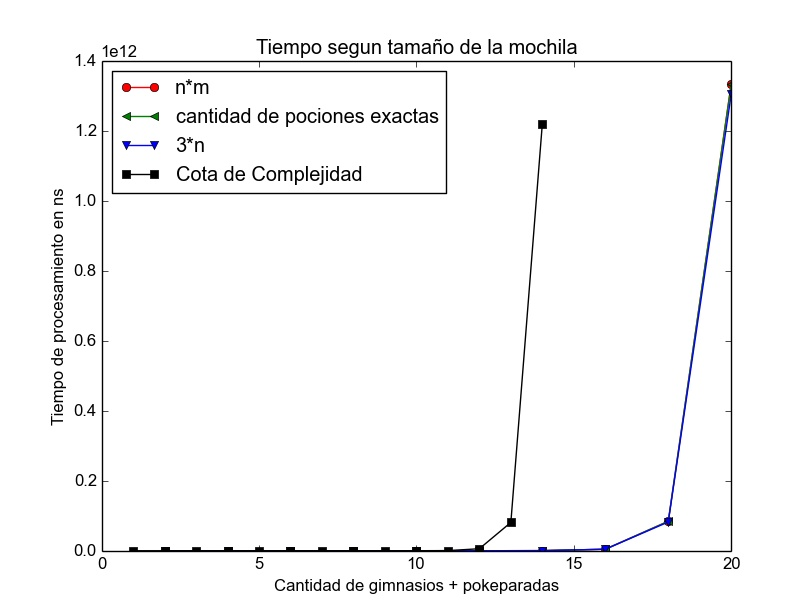
\includegraphics[width=0.7\columnwidth]{imagenes/exp1_ej1.jpeg}
        \caption{}
      \end{center}
  \end{figure}

  % Para cada matriz puede observarse que a medida que crece la cantidad de paredes que se pueden derribar, también crece el tiempo que toma cada ejecución del programa, que era el comportamiento que se esperaba. Si bien el algoritmo de BFS corta la ejecución en cuanto encuentra el destino (en caso de poder encontrarse), no se observa una mejoría cuando se utiliza una cantidad mayor de paredes que se pueden destruir a la cantidad de nodos, debido a que en la construcción del grafo se toman en cuenta todos los niveles (cantidad de paredes), por lo que esa parte del algoritmo ya toma $O(FCP)$. Por esta razón es que el tiempo de ejecución no se mantiene constante una vez que se toma una cantidad de paredes mayor al total de nodos. El algortimo como se puede observar también tarda menos en ejecutar cuando en la matriz no hay ninguna pared y el origen y el destino están uno al lado del otro, como se esperaba. Este es el mejor caso. Los casos en los cuales había una cantidad de paredes igual a la mitad de nodos y éstas estaban en posiciones horizontales y verticales fueron aún peor que en el caso que son todas paredes. Esto puede explicarse debido a que el algoritmo de BFS inspecciona algunos vecinos que en el caso de que son todas paredes no puede ya que no tiene ningún camino que pueda pasar sin romper paredes.
  % Podemos notar como la cota de complejidad cumple, aunque no de manera exacta, su función para estos experimentos.


  % Luego se realizó otro tipo de experimento en el cual se utilizaron otras cinco matrices pero con tamaño y paredes dispuestas de manera aleatoria. Estas matrices fueron generadas usando la librería random de la STL con distribución uniforme. Este experimento se corrió bajo las mismas circunstancias que el otro experimento. Se corrieron 100 casos para cada una de las matrices, considerando que se pueden romper desde 0 a 99 paredes. Además también cada uno de los casos se repitió 100 veces y se tomó el promedio. Los resultados que se obtuvieron son los siguientes:

  \begin{figure}[H]
      \begin{center}
        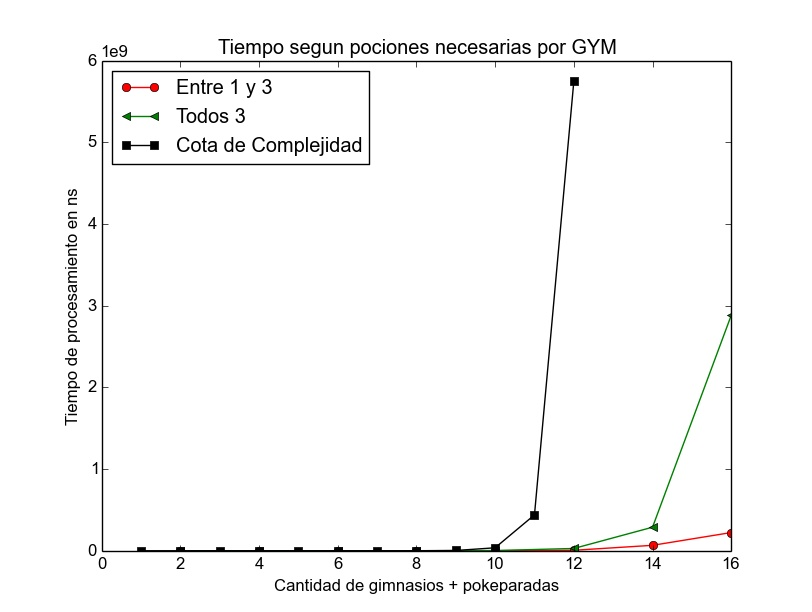
\includegraphics[width=0.7\columnwidth]{imagenes/exp2_ej1.jpeg}
        \caption{}
      \end{center}
  \end{figure}

  % Se observa también como el tiempo de ejecución aumenta a medida de que se pueden romper más paredes para cada una de las matrices. Por lo general, los casos en los cuales la matriz tiene menos filas y columnas presentan un tiempo de ejecución menor pero pueden observarse que igualmente también depende de la cantidad de paredes que haya en la matriz. Para estos casos, la cota propuesta acota mejor de manera superior a todos los casos.

  \begin{figure}[H]
      \begin{center}
        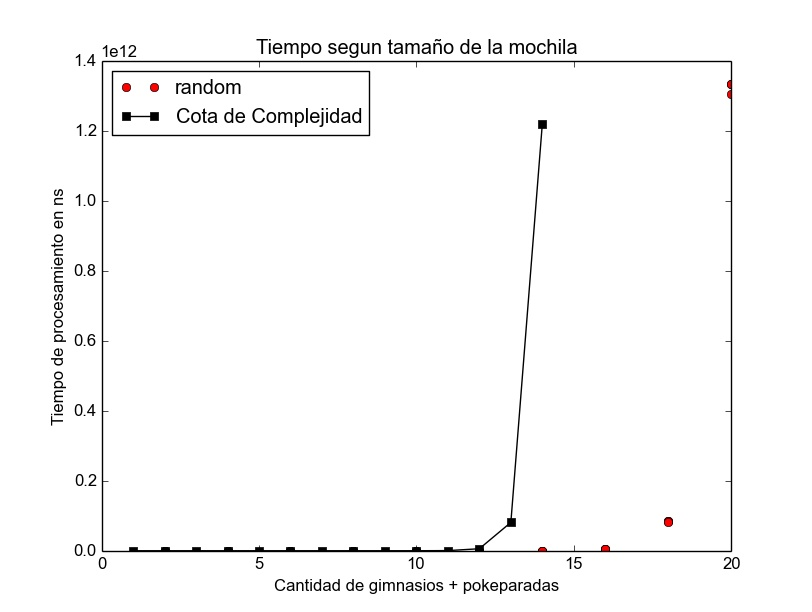
\includegraphics[width=0.7\columnwidth]{imagenes/exp3_ej1.jpeg}
        \caption{}
      \end{center}
  \end{figure}


% \newpage
% \section{Ejercicio 2: Heurística constructiva golosa}

  % \begin{figure}[ht]
  %   \begin{center}
  %     \includegraphics[width=0.5\columnwidth]{imagenes/pacman.png}
  %     \caption{Perdidos y con poca fuerza}
  %   \end{center}
  % \end{figure}

    % 1. Describir detalladamente el problema a resolver dando ejemplos del mismo y sus soluciones.
    \subsection{Descripción del problema y solución propuesta}
        En este punto, se pidió realizar un algoritmo basado en una heurística constructiva golosa que resuelva el problema en cuestión. El mismo al tratarse de una heurística puede no dar la solución óptima, y puede no devolver una solución aunque la misma exista.

    % 2. Explicar de forma clara, sencilla, estructurada y concisa, las ideas desarrolladas para la resolución del problema. Utilizar pseudocódigo y lenguaje coloquial (no código fuente). Justificar por qué el procedimiento resuelve efectivamente el problema.
        Se decidió utilizar como heurística golosa para resolver esta variante del TSP, la técnica del vecino más cercano. La misma consiste en lo siguiente: en cada momento, el algoritmo selecciona como próximo nodo a visitar el que se encuentre a menor distancia del actual. Como en este caso puede ocurrir que no se pueda ir al nodo más cercano debido a que no se poseen las suficientes pociones (para enfrentarlo en caso de que sea un gimnasio), el algoritmo selecciona al nodo más cercano que se pueda ir. El funcionamiento es el siguiente: se busca un nodo inicial al que se pueda ir, ya sea porque alcanzan las pociones (para el caso de un gimnasio) o porque se pueden recibir pociones (porque la mochila no está llena). Una vez identificado un nodo inicial se busca la estación (gimnasio o pokeparada) más cercana a la que se pueda ir. Este procedimiento se repite sucesivamente hasta que se visiten todos los gimnasios o hasta que no se pueda ir a ningún nodo (porque la mochila está llena y no alcanza para ir a ningun gimnasio o porque no quedan mas pokeparadas y no se puede vencer a ningún gimnasio).
        Este método no garantiza que la solución encontrada sea óptima ya que puede pasar que se recorran pokeparadas innecesariamente sólo por el hecho de estar próximas entre sí y además puede ser que no se encuentre una solución aunque si haya alguna porque se pueden desperdiciar pociones en una instancia similiar a la anterior mencionada.
        Basándonos en la técnica del vecino más cercano, las intancias en los cuales los gimnasios estén cerca uno de los otros y se tenga la cantidad suficiente de pociones para ir a ellos, van a ser resueltas de manera muy cercana a la óptima. Los casos en los cuales las pokeparadas estén muy cercas unas de otras, van a tener peores resultados con esta técnica ya que se van a recorrer nodos que en su mayoría son innecesarios, ya que se podría directamente pasar por los gimnasios.

        \subsection{Detalles implementativos}
            Las clases y estructuras utilizadas en el algoritmo son las mismas que las del primer ejericio. El algoritmo propuesto para la heurísitica golosa es el siguiente: 

            \begin{codesnippet}
            \begin{verbatim}
solverEj2(vector<Estacion> estaciones, vector<vector<double> > distancias, cantidad_gimnasios,
          cantidad_pokeparadas, mochila_size)
  
  vector<int> camino_nulo
  solucion = (-1,-1,camino_nulo)
  si puedo ir a algun nodo inicial
      vector<Estacion> visitados
      id = donde_voy(estaciones, 0, mochila_size)
      index = indice_estacion_con_id(id, estaciones)
      visitados.agregar(estaciones[index])
      potasActuales = (si es gimnasio o mochila_size >3)
                         estaciones[index].potas
                      si no 
                         mochila_size 
      estaciones.borrar(estaciones.begin() + index)
      greedy_capturar_gimnasios(estaciones,distancias,cantidad_gimnasios,cantidad_pokeparadas,
                                mochila_size,visitados,potasActuales,id,solucion)
  
  devolver solucion

greedy_capturar_gimnasios(vector<Estacion> estaciones, vector< vector<double> > distancias, 
                          cantidad_gimnasios, cantidad_pokeparadas, mochila_size, 
                          vector<Estacion> visitados, potasActuales, id_estacion_actual, 
                          tuple<double,int,vector<int> > soluciones)
  i = 0
  mientras i < (n+m) y no es_solucion(estaciones)
    ordenar(estaciones, distancias, id_estacion_actual)
    id = donde_voy(estaciones, potasActuales, k)
    si id es igual a -1
       i = n + m
    si no
       index = indice_estacion_con_id(id, estaciones)
       visitados.agregar(estaciones[index])
       potasActuales += estaciones[index].potas
       estaciones.borrar(estaciones.begin() + index)
       id_estacion_actual = id
       i = i + 1
  fin mientras
  si es_solucion(estaciones)
      distancia = distancia_acumulada(visitados,distancias)
      vector<int> camino

      for (u = 0 hasta visitados.size() - 1)
        camino.agregar(visitados[u].id)

      soluciones = (distancia, visitados.size(), camino)

ordenar(vector<Estacion> estaciones, vector< vector<double> > distancias, id_estacion_actual)

  vector<int> ids_vistos
  ids_vistos.agregar(id_estacion_actual)
  for (i = 0 hasta estaciones.size() - 1)
    id_mas_cercano = id_mas_cercano_que_no_viste(distancias[id_estacion_actual], 
                                                 ids_vistos, estaciones)
    ids_vistos.agregar(id_mas_cercano)
    swap(id_mas_cercano, i, estaciones)
            \end{verbatim}
            \end{codesnippet}





            El algoritmo lo primero que realiza es obtener el id de una estacion inicial. El mismo es obtenido llamando a una función \textit{donde voy}. Esta función recibe por parámetros un vector con las estaciones, la cantidad de pociones que se posee y el tamaño de la mochila, y recorre las estaciones y por cada una de ellas se fija si alcanzan las pociones para enfrentarse al gimnasio (en caso que la estacion sea un gimnasio) o si puede recibir las pociones (en caso de ser una pokeparada y no tener la mochila llena). De haber alguna, devuelve el id de la primera estacion que encuentra. En caso contrario la función devuelve -1, indicando que no hay ninguna estación a la cual se puede ir. Si la función devuelve -1 no se puede tomar ninguna estación inicial por lo que simplemente se devuelve lo solicitado en el enunciado (-1). En caso contrario se utiliza el id y se recupera el índice de la estacion en el vector de estaciones llamando a la función \textit{indice estacion con id} para luego agregar al vector de visitados la estacion correspondiente a este índice. De esta forma, tenemos el primer nodo (estación) visitado. Se definen las pociones actuales como las pociones de esta estacion (en el caso de que sea un gimnasio o que el tamaño de la mochila sea mayor a 3) o como el tamaño de la mochila (en caso contrario). Se borra del vector de estaciones la estación visitada, para indicar que la misma ya fue visitada. Finalmente se llama a la función \textit{greedy capturar gimnasios} la cual realiza un procedimiento similar al anteriormente mencionado hasta que termine de recorrer todos los gimnasios (en caso de que pueda). La función \textit{greedy capturar gimnasios} recibe el vector de estaciones, un vector de vector de distancias (que contiene todas las distancias desde todas las estaciones a todas las demás, el mismo que se utilizó en el primer ejercicio), la cantidad de gimnasios (n), la cantidad de pokeparadas (m), el tamaño de la mochila (k), el vector de estaciones visitadas, las pociones actuales que se posee, el id de la estacion actual y una tupla que contiene la distancia total, la cantidad de estaciones que hay que recorrer, y un vector con los ids en orden de las estaciones que hay que recorrer.
            En la función hay un ciclo que se ejecuta n + m veces (la cantidad de estaciones total), mientras no se haya encontrado una solución. Para saber si se encontró una solución o no, se recorren todas las estaciones para verificar que no haya ningún gimnasio sin visitar. En el cuerpo del ciclo se realiza el ordenamiento de las estaciones, la parte fundamental de la heurística greedy. El mismo consiste en una función \textit{ordenar} que recibe por parámetro el vector de estaciones, el vector de vector de distancias, y el id de la estación actual en la cual se está analizando. Lo que hace la función es recorrer el vector de distancias de la estación actual y ordena el vector de estaciones de acuerdo a este vector de distancias. De esta manera en cada iteración el vector de estaciones queda ordenado por distancia relativa a la estación actual que se está analizando. Luego del ordenamiento se llama nuevamente a la función que devuelve el id de la siguiente estación que hay que visitar. Como ahora el vector de estaciones está ordenado y se recorre de adelante para atrás, esta función va a devolver el id de la estación más cercana a la que se puede ir. Si devuelve -1, se actualiza el índice del ciclo con el valor n + m para que termine ya que no se puede avanzar. Si no, se recupera el índice de la estación con ese id, se agrega la estación nueva al vector de visitados y se actualizan las pociones actuales, de acuerdo al tipo de estación que se visitó. Se borra la estación del vector de estaciones para que no sea considerada nuevamente y se actualizan el id de la estación actual con el nuevo id y se incrementa el índice del ciclo. Luego del ciclo, se verifica que sea una solución lo que se haya encontrado y en caso de serlo se suma las distancias de todos los nodos visitados y se actualiza la tupla de solucion con la distancia total, la cantidad de estaciones visitadas y el camino realizado, para que al retornar de la función la tupla solución contenga la solución al problema. 

            % 3. Deducir una cota de complejidad temporal del algoritmo propuesto y justificar por qué el algoritmo cumple la cota dada. Utilizar el modelo uniforme.
    \subsection{Complejidad teórica}

      La función que resuelve el problema (solverEj2) realiza las siguientes operaciones con el siguiente costo temporal: La inicialización del vector y la tupla se realizan en $O(1)$. La función que es llamada \textit{donde voy} tiene complejidad temporal $O(n+m)$ ya que recorre todas las estaciones analizando en $O(1)$ si se puede ir a alguna de ellas. La función que devuelve el índice de la estación con un id determinado también tiene complejidad $O(n+m)$ ya que recorre todo el vector de estaciones en el peor caso. Los agregar y borrar del vector se realizan en $O(1)$ amortizado. Finalmente falta sólo analizar la complejidad de la función \textit{greedy capturar gimnasios} y con ella determinar la complejidad resultante de solverEj2. 
      Esta última función tiene un ciclo que se ejecuta en el peor caso $n+m$ veces. En el cuerpo del ciclo se llama a la función ordenar la cual recorre el vector de estaciones (en $O(n+m)$) y en cada iteración recupera el id del más cercano. Para recuperar este id, la función \textit{id mas cercano que no viste} recorre todas las distancias de las demas estaciones en $O(n+m)$, preguntando en cada caso si esa estación se vio o no (en $O(n+m)$). Luego ordenar en cada iteración realiza el swap correspondiente de estaciones, que para el mismo necesita recorrer nuevamente todas las estaciones ($O(n+m)$) para poder recuperar el id de la estacion que quiere intercambiar. En conclusión, ordenar realiza en el peor caso $O(n+m)*O(n+m)*O(n+m)$ operaciones resultanto en una complejidad temporal de $O(n+m)^3$. 
      Después de ordenar, la función greedy llama a la función donde voy ($O(n+m)$). Se realiza una comparación con el id devuelto de esta función en $O(1)$ y si es distinto de -1 se llama a la función que devuelve el índice de la estación ($O(n+m)$). Las otras operaciones del ciclo se realizan en tiempo cosntante ($O(1)$). 
      Después del ciclo se pregunta si se encontró o no solución chequeando el vector de estaciones ($O(n+m)$ en el peor caso). La distancia acumulada se calcula iterando todos las estaciones vistas ($O(n+m)$ en el peor caso) y se arma el camino ($O(n+m)$ en el peor caso). En definitiva el ciclo es el que domina la complejidad de la función ya que por lo dicho realiza $O(n+m)*O(n+m)*O(n+m)*O(n+m) = O(n+m)^4$ operaciones.
      Por lo tanto la función solverEj2 tiene una complejidad temporal teórica de $O(n+m)^4$. La complejidad espacial es la misma que la del ejercicio 1 ya que se utiliza para representar las distancias un vector con tamaño igual a la cantidad de estaciones en el cual en cada posición se tienen las distancias a todas las demás estaciones, lo que da un total de $O((n+m)^2)$. 

      \subsection{Comportamiento del algoritmo}
      El algoritmo al tratarse de una heurística no devuelve una solución exacta en todos los casos. A continuación se procede a realizar un análisis del comportamiento del algoritmo para distintos tipos de instancias. El peor caso es que el algoritmo no devuelva ninguna solución aunque la misma exista. Esto puede suceder en instancias en las cuales las pokeparadas están muy próximas entre sí por lo que al algoritmo al basarse en el vecino mas cercano las va a recorrer a todas (siempre y cuando el tamaño de la mochila sea lo suficientemente grande como para recuperar pociones en todas las pokeparadas) antes que los gimnasios. De esta forma puede suceder que haya pociones que se desperdicien porque cada pokeparada devuelve 3 pociones y si en la mochila caben sólo 1 o 2 pociones se van a descartar 2 o 1 pocion respectivamente. De esta forma puede suceder que debido a ese descarte no alcancen para vencer a un gimnasio. La siguiente instancia es un ejemplo que cumple con esas características: 

      \begin{codesnippet}
            \begin{verbatim}
2 3 7
1 1 2
2 2 6
7 7
8 8
9 9

\end{verbatim}
            \end{codesnippet}


      Para este caso el algoritmo propuesto no devuelve solución. Lo que realiza es lo siguiente: toma la primer estación a la que puede ir que en este caso es la que se encuentra en (7,7). Al tratarse de una pokeparada recibe 3 pociones. Luego la estación mas cercana a la que puede ir es (8,8) que es otra pokeparada en donde recibe otras 3 pociones (en total tiene 6). Luego la próxima estación más cercana es otra pokeparada (9,9) de la cual solo puede recibir 1 pocion (porque el tamaño de la mochila es 7 y ya tenia 6). Estas dos pociones que "desperdicia" son las que hacen que despúes no le alcance para vencer a los dos gimnasios. La última estación a la que visita es (2,2) por proximidad y en esta gasta 6 pociones, quedandole una sola disponible en la mochila. Finalmente le queda una única estación (el gimnasio que se encuentra en 1,1) pero que no puede vencer porque le falta una poción y no quedan mas pokeparadas sin recorrer. De esta forma el algoritmo retorna que no hay solución cuando si existe y la óptima es la siguiente: 

      D = 25.4558 k = 5 i = 5 4 2 3 1

      Es decir se pueden recorrer las estaciones (8,8) y (9,9) obteniendo 6 pociones, enfrentar el gimnasio que se encuentra en (2,2), usando las 6 pociones, ir a la pokeparada (7,7) y finalmente venciendo al gimnasio en (1,1).

      Además de no devolver la solución hay casos en donde el algoritmo si devuelve una solución pero la misma no es óptima y hace que se recorran todas las estaciones, como por ejemplo el siguiente:

\begin{codesnippet}
            \begin{verbatim}
3 3 7
1 1 1
2 2 1
3 3 1
7 7
8 8
9 9

\end{verbatim}
            \end{codesnippet}


      En este caso el algoritmo devuelve lo siguiente:

      D= 14.1421 k= 6 i= 4 5 6 3 2 1

      Es decir recorre todas las pokeparadas y después todos los gimnasios cuando el óptimo es ir a la pokeparada en (7,7) y despues a los gimnasios (3,3),(2,2) y (1,1). 

      Hay casos igualmente que el algoritmo devuelve la solución óptima como por ejemplo en el siguiente:

      \begin{codesnippet}
            \begin{verbatim}
3 3 6
1 1 1
2 2 1
3 3 1
4 4
8 8
9 9

\end{verbatim}
            \end{codesnippet}


      En este caso el algoritmo primero recorre la estación (4,4) que es una pokeparada de donde obtiene 3 pociones y después por proximidad visita las estaciones (3,3),(2,2) y (1,1) ya que puede enfrentar a todos los gimnasios porque todos requieren solo 1 pocion. 

\subsection{Experimentación}

      Los experimentos que realizamos para observar los tiempos de ejecución del algoritmo en función del tamaño de entrada consistieron en el análisis de casos que contemplan:

      \begin{itemize}
        \item Configuraciones de valores que no están en la cota de complejidad
        \item Configuraciones de valores que sí están en la cota de complejidad, dejando fijos los demás
        \item Casos random generados a partir de la librería Random de la STL de C++ utilizando distribución uniforme
      \end{itemize}

      Para todos los casos, el algoritmo se ejecutó 30 veces con cada instancia para intentar tener la mayor presición posible en cuanto a tiempo de ejecución.

      \subsubsection{Analisis de configuraciones de valores que están en la cota de complejidad}
      En esta instancia generamos entradas que aumentaban linealmente de 1 a 10 la cantidad de pokeparadas y gimnasios, variando el tamaño de la mochila y marcando a cada gimnasio con la cantidad de pociones necesarias igual al numero de linea en el input (para el gimnasio 3, se piden 3 pociones). Además, las ubicaciones de cada estación se setearon cada una a distancia 1 de la anterior y la siguiente: para la estación $i$ la ubicación es ($i$,$i$).

      Algunos ejemplos para el input de este experimento son los siguientes:

\newpage
\section{Ejercicio 3: Búsqueda Local}
    % 1. Describir detalladamente el problema a resolver dando ejemplos del mismo y sus soluciones.
    \subsection{Descripción del problema y solución propuesta}

    \par Una vez obtenida una heurística greedy para resolver nuestra variante de TSP, utilizamos una \textbf{Búsqueda Local} para analizar una mayor cantidad de soluciones posibles. Es decir, dada una solución inicial S (obtenida de aplicar a una instancia de entrada, el algoritmo heurístico implementado en el Ejercicio 2) se obtienen los vecinos de S, es decir, un “vecindario“ de soluciones. Y de este vecindario, se obtiene el vecino cuya solución mejore a S. Luego se realiza una búsqueda local sobre este vecino. 
    \par Sea V este vecindario, $\forall S^{*}\in V, S^{*} = h(S)$ h es una función que obtiene un vecino a partir de S, perteneciente a V. En otras palabras, h altera la solución S para encontrar una solución parecida que pueda mejorar el resultado. Por otro lado, se cuenta con una función f que da valor a cada una de las soluciones. En nuestro caso, sean S y $S^{'}$, diremos que una solución S es mejor que $S^{'}$ si $f(S) < f(S^{'})$. Luego para cada $S^{*}\in V$, se evalúa f($S^{*}$). 
    \par Dado V el conjunto de vecinos del Vecindario y S la solución original, si $\forall S^{*}\in V$, $f(S) < f(S^{*})$  se devuelve la solución S. En caso contrario, se recorre el vecindario de soluciones y se aplica nuevamente la búsqueda local sobre el $S^{*} \in Vecindario $ cuyo valor sea el mínimo, y se reemplaza a S por $S^{*}$. Esto se repite hasta que no haya un $S^{*}$ que cumpla $f(S^{*}) < f(S)$. Una vez que esto ocurre, se devuelve S. 
    \par De esta manera, a partir de una solución se estará explorando sus vecinos, y la búsqueda local se detendrá al hallar una mínimo local.

    \subsubsection{Vecindad A}

    \par Se realiza una búsqueda local aplicado a nuestro problema de la siguiente manera. La solución inicial S, se obtiene de aplicar la heurística del vecino más cercano (explicada en el Ejercicio 2) a los parámetros pasados por entrada. En nuestro caso, S consiste en una tupla con distancia, recorrido y cantidad de estaciones.
    \par Una vez obtenida esta solución, contamos con la función \textbf{h} la cual generará la primer vecindad. En este caso, la función $h$ se denomina \emph{dameVecindario}, y se encarga de intercambiar únicamente las \emph{pokeparadas} dentro del recorrido de S. Por cada intercambio generado, se guarda este nuevo recorrido en un vector.

    \begin{codesnippet}
    \begin{verbatim}
    vector<vector<int>> dameVecindario(lista<Estacion> estaciones, lista<int> recorrido)
        vector<vector<int>> vecindario;
        Para i = 0...recorrido.size() - 1
            Si la estacion pasada en el recorrido[i] no es gimnasio
                Para j = i+1 ... recorrido.size()
                    Si la estacion pasada en el recorrido[j] no es gimnasio
                        Creo un vector estadoAux <-- recorrido
                        Hago swap entre i y j en estadoAux
                        vecindario.push_back(estadoAux);
                    Fin si
                Fin
            Fin Si
        Fin
        Devolver vecindario
    \end{verbatim}
    \end{codesnippet}

    En nuestro caso, una solución es mejor que otra si una logra conquistar todos los Gimnasios recorriendo menor distancia que la otra, manteniendo siempre el invariante de no pasar por la misma estación más de una vez. 
    Una vez obtenido el vecindario, la función f evalúa cada solución. En nuestro caso f se llama “dameDistancia“ y se encarga de calcular la distancia de cada solución obtenida, guardándola en el vector vecindario. Luego compara cada una con S. 
    \par Si la distancia de algún recorrido nuevo en el vecindario (por ejemplo $S^{*}$) es menor que la distancia que recorrió S, se repite el ciclo de búsqueda local sobre algún $S^{*}$. Caso contrario, se devuelve la solución S con su recorrido, su distancia y la cantidad de estaciones por donde pasó.

   \subsubsection{Vecindad B}

    \par A diferencia de la Vecindad A, la función h del vecindario B, se llama “dameVecindario2“ y se encarga de intercambiar únicamente los \emph{gimnasios} dentro del recorrido S, siempre que cada intercambio de gimnasios en el recorrido no cause que alguno de los gimnasios no pueda ser conquistado.

    \begin{codesnippet}
    \begin{verbatim}
    vector<vector<int>> dameVecindario2(lista<Estacion> estaciones, lista<int> recorrido,
                                        matriz<double, double> distancias, int k)
        vector<vector<int>> vecindario;
        Para i = 0...recorrido.size() - 1
            Si la estación pasada en el recorrido[i] es gimnasio
                Para j = i+1 ... recorrido.size()
                    Si la estación pasada en el recorrido[j] es gimnasio
                        Creo un vector estadoAux <-- recorrido
                        Hago swap entre i y j en estadoAux
                        Si el recorrido sigue siendo válido (se conquistan todos los gimnasios)
                            vecindario.push_back(estadoAux);
                        Fin si
                    Fin si
                Fin
            Fin Si
        Fin
        Devolver vecindario
    \end{verbatim}
    \end{codesnippet}
    
    \par El resto del procedimiento es equivalente al explicado para la búsqueda local que incluye el Vecindario A.
   
    \subsection{Complejidad teórica}
        Para la complejidad teórica, debemos mostrar por cada iteración de la búsqueda local cual será la cota asintótica. 
        \par Para empezar, hablaremos de la \textbf{Vecindad A}. Como fue explicado anteriormente, se encarga de crear las posibles combinaciones de intercambiar la posición de las pokeparadas en el recorrido. Para calcular la complejidad en cada iteración de la búsqueda local, sean N los nodos gimnasio y M los nodos pokeparadas, se deben tener en cuenta:

        \begin{itemize}
            \item Para ingresar a la búsqueda local, se copia el vector recorrido, de la solución inicial S, esto cuesta \ord(N+M).
            \item Luego se entra al ciclo principal de búsqueda local que en el peor de los casos tendrá M! iteraciones. Esto se debe a que, dado que en cada iteración se permutan ciertas pokeparadas, en el peor de los casos, siempre encuentra una solución mejor. Va a tomar \ord(M!) iteraciones recorrer todas las permutaciones posibles.
            \item Dentro del ciclo principal, se busca el vecindario de una solución. Para esto se llama a la función \emph{dameVecindario} con el vector \emph{recorrido}.
            La misma función, recorre el vector hasta que el i-ésimo elemento sea pokeparada. Luego recorre el vector restante, desde i+1 hasta recorrido.size()-1. Es decir, la complejidad del ciclo, siendo r la cantidad de estaciones del recorrido, es de 
            \[
            \ord(\sum_{i=0}^{r-1} i)
            \] 
            
            \par Que dada la progresión aritmética,
            \[
            \sum_{i=0}^{r-1} i = r * (r - 1)
            \]

            \par Esto quedaría,
            \[
            \ord(r * (r - 1) / 2)
            \]
            \par Además, como mencionamos anteriormente, el tamaño del recorrido en el peor caso es \ord(N+M). Luego,
            \[
            \ord((N+M))*(N+M-1)/2)
            \]

            Luego, dentro del ciclo, se copia el vector recorrido en un vector \emph{estadoAux}, la copia del vector es \ord(N+M), y si esto se realiza en cada ciclo,
             \[
            \ord(((N+M))*(N+M-1)/2)*(N+M)) = \ord((N+M)^{3})
            \]

            \item Una vez obtenido el vecindario se recorre el vector \emph{vecindario} y por cada vecino se itera sobre su recorrido calculando la distancia. Dado que las iteraciones dentro de \emph{dameVecindario}, empieza en la i-ésima pokeparada, y por cada elemento a partir del i+1, que también sea pokeparada, se genera un intercambio de elemento dentro del vector, entonces la cantidad de vecinos distintos serán,
            \[
             $\sum_{i=0}^{M-1} i = M(M-1)/2$
            \] 
            Luego la cantidad de vecinos diferentes, es decir el tamaño total del vector vecindario es de $M(M-1)/2$. Calcular la distancia, implica por cada vecino, recorrer todo el vector \emph{recorrido}, esto es \ord(N+M). Esto lo realiza para los M(M-1)/2 vecinos. Es decir
            \[
                \ord((M(M-1)/2)*(N + M)) = \ord(M^{2}*(N+M))
            \]
            \item Finalmente, dada la solución, se genera una tupla en \ord(1) y se devuelve esta solución.

        \end{itemize}

        Es decir, la complejidad quedaría
        \[
            \ord(N+M) + \ord(M!)*(\ord((N+M)^{3}) + \ord(M^{2}*(N+M)) =
        \]
        \[
            \ord(M!)*(\ord((N+M)^{3}) + \ord(M^{2}*(N+M)) =
        \]
        \[
            \ord(M!*((N+M)^{3} + M^{2}*(N+M))) =
        \]

        \[
            \ord(M!*((N+M)^{3}))
        \]
        Pues $\ord(M^{2}*(N+M)) = \ord((N+M)^{3})$

        Finalmente, la complejidad total es de
        \[
            \ord(M!*((N+M)^{3}))
        \] 


        \par Por otro lado, hablaremos de la complejidad del vecindario B. La misma, comparte gran parte de la complejidad del vecindario A. Por lo que se nombrarán las partes relevantes del algoritmo de búsqueda local con el vecindario B.
        \begin{itemize}
            \item Para ingresar a la búsqueda local, se copia el vector recorrido, de la solución inicial S, esto cuesta \ord(N+M).
            \item Luego, busca las permutaciones de los gimnasios, por lo que, el ciclo principal de la búsqueda local, tendrá en el peor de los casos N! iteraciones. Es decir, si intercambiar los gimnasios siempre genera una solución posible, como en cada iteración se permutan algunos gimnasios, en el peor de los casos, siempre encuentra una solución mejor dentro del vecindario. Luego esto tomará \ord(N!) iteraciones recorrer todas las permutaciones posibles.
            \item Dentro del ciclo principal, se busca el vecindario de la solución. Para esto, se llama a la función \emph{dameVecindario2} con el vector \emph{recorrido}. Hace las mismas iteraciones que en el vecindario A, es decir 
            \[
                \ord((N+M)*(N+M-1)/2)
            \]

            Con la diferencia que, sea r = recorrido.size(), copiar el vector\emph{recorrido} en \emph{estadoAux} cuesta \ord(r), y además debe chequear que el nuevo recorrido es válido. Para esto, recorre nuevamente el vector \emph{estadoAux}, viendo que se cumplan diferentes condiciones. Luego como fue mencionado, dado que se copia \emph{recorrido} en \emph{estadoAux} y $r = \ord(N + M)$, entonces $estadoAux.size() = r = \ord(N+M)$. Luego copiar el vector es \ord(N+M) y recorrer el vector estadoAux, es 
            \[
                \ord(2*(N+M)) = \ord(N+M)
            \]

            Esto quiere decir que, por cada ciclo de \emph{dameVecindario2}, debe copiar el vector y chequear que sea válido. Y las iteraciones de esta función eran \ord((N+M)*(N+M-1)/2). Luego quedaría \ord((N+M)*(N+M-1)/2*(N+M)), entonces
            \[
                \ord((N+M)*(N+M-1)/2*(N+M)) = \ord((N+M)^3)
            \]

            \item Luego una vez obtenido el vecindario, se calcula al igual que en el \textbf{vecindario A} las distancias de cada vecino en $\ord(M^{2} * (N+M))$
            \item Por último en $\ord(1)$ se genera una tupla como solución y se devuelve.

            Entonces, la complejidad quedaría
        \[
            \ord(N+M) + \ord(N!)*(\ord((N+M)^{3}) + \ord(M^{2}*(N+M)) =
        \]
        \[
            \ord(N!)*(\ord((N+M)^{3}) + \ord(M^{2}*(N+M)) =
        \]
        \[
            \ord(N!*((N+M)^{3} + M^{2}*(N+M))) =
        \]
        \[
            \ord(N!*((N+M)^{3}))
        \]
        Pues $\ord(M^{2}*(N+M)) = \ord((N+M)^{3})$

        Finalmente, la complejidad total es de
        \[
            \ord(N!*((N+M)^{3}))
        \] 

        \end{itemize}
    % 4. Dar un código fuente claro que implemente la solución propuesta. Se deben incluir las partes relevantes del código como apéndice del informe impreso entregado.

    \subsection{Detalles Implementativos}

    
    Las clases y estructuras utilizadas en el algoritmo son las mismas que las del primer ejercicio. El algoritmo propuesto para las búsquedas locales es el siguiente: 

            \begin{codesnippet}
            \begin{verbatim}

solucion busquedaLocal(vector<int> recorridoInicial, vector<Estacion> estaciones, 
    matriz<double> distancias, double distancia, bool elegirVecindario)
    
    matriz<int> vecindario;
    double distanciaMinima;
    double distanciaAux;
    int proximoEstado;
    bool hayanSoluciones = true;
    vector<int> recorrido = recorridoInicial;

    mientras hayanSoluciones
        vecindario = dameVecindario(estaciones, recorrido, elegirVecindario)
        //obtiene un vecindario de soluciones
        
        proximoEstado = -1;

        si el vecindario no es vacío
            
            distanciaMinima = distancia;
            
            //Busco algún vecino con distancia mas chica
            para cada vecino entre 0 y tam(vecindario)
                
                distanciaAux = dameDistancia(vecindario[vecino], distancias);
                //obtiene las distancia recorridas de la solución vecino-ésima

                si distanciaAux < distanciaMinima
                    distanciaMinima = distanciaAux;
                    proximoEstado = vecino;
                fin si
            fin para cada
        fin si
    
        si proximoEstado > -1
            recorrido = vecindario[proximoEstado];
            distancia = distanciaMinima;
        sino
            hayanSoluciones = false;
        fin si

    fin mientras

    devolver solucion (distancia, tam(recorrido), recorrido);
fin busquedaLocal
            \end{verbatim}
            \end{codesnippet}


            El algoritmo obtiene una primera solución \textbf{recorridoInicial} en base al algoritmo greedy goloso implementado en el Ejercicio 2.
            \par Luego, busca un vecindario de soluciones en base a la solución obtenida (dado el parámetro \textbf{elegirVecindario}, se elige uno de los dos tipos de vecindarios).
            \par Se obtiene la mejor solución del vecindario, es decir, la que menor distancia recorre. Llamémosla S.
            \par Por último se vuelve a repetir el procedimiento, buscando un vecindario de soluciones a partir de la solución S.

            \par Todo este procedimiento se repite hasta que el vecindario de soluciones no contenga ninguna solución mejor que la solución ya obtenida.


    % 5. Realizar una experimentación computacional para medir la performance del programa implementado. Usar un conjunto de casos de test en función de los parámetros de entrada, con instancias aleatorias e instancias particulares (de peor/mejor caso en tiempo de ejecución, por ejemplo). Presentar en forma gráfica una comparación entre los tiempos medidos y la complejidad teórica calculada y extraer conclusiones.
    \subsection{Experimentación}
    Los experimentos realizados permiten observar las diferentes calidades de solución para ambos vecindarios, es decir, en el primer experimento se comparó junto al resultado exacto dado por backtracking, qué vecindario devolvía la menor distancia posible, mientras que en el segundo experimento, se comparó las soluciones devueltas por búsqueda local contra las devueltas por el algoritmo greedy. Además en ambos experimentos, se comparó la performance de cada vecindario, es decir, se calculó el tiempo en ns por cada uno. En cuanto a instancias, en el primer experimento, utilizamos instancias particulares que serán explicadas en él. Mientras que en el segundo, se generó un mayor número de instancias random, asegurándonos que tengan solución.



        \subsubsection{Experimento 1} 

            Como hipótesis mantuvimos que, dado que en el vecindario A se intercambian pokeparadas, el campo de soluciones recorridas por él es mayor al del vecindario B, debido a que, al intercambiar pokeparadas de una solución esta sigue siendo solución, mientras que en el vecindario B, por cada intercambio de gimnasios, debe filtrar aquellos que no devuelven una solución válida, teniendo menos margen para generar vecinos. Entonces, \textbf{en general}, esto permite que el vecindario A, obtenga mejores soluciones que el B. 

        \subsubsection{Experimento 1: Calidad de resultados} 

            Para experimentar acerca de la calidad de los resultados de ambas vecindades, se generaron distintas comparaciones. 

            \begin{itemize}
                \item Por un lado, se comparó cada vecindario por separado con backtracking. Para esto se generaron 66 instancias, de las cuales, las primeras 20 instancias cumplen las mismas condiciones mencionadas en \textbf{Ejercicio 1: Experimento 1}. Por otro lado las siguientes 16 instancias  cumplen con las mismas condiciones que menciona el \textbf{Ejercicio 1: Experimento 2} y por último, fueron generadas 30 instancias que por cada una se aumenta en 1 la cantidad de gimnasios y pokeparadas, manteniendo siempre que la distancia entre cada estación es 1.
 
                \item Por otro lado, se compararon los tres algoritmos juntos, corriendo 16 instancias creadas también manualmente. Por cada instancia, aumentamos de la misma manera la cantidad de gimnasios, pokeparadas y capacidad de las mochilas. Al igual que la anterior comparación, se mantuvo que la distancia entre cada estación es 1.
            \end{itemize}

             En ambas comparaciones, por cada algoritmo, se corrió 30 veces la misma instancia, sacando un promedio de la distancia devuelta. Luego, en función de la cantidad de estaciones (n+m), se comparó qué distancias devolvían. Los demás valores de entradas son los mismos que se utilizaron para el experimento de performance realizado en el Ejercicio 2.
			 
			 \par A continuación en los siguientes gráficos se puede observar la calidad de resultado de cada vecindario en comparación con el algoritmo exacto.

\blindtext

\begin{figure}[H]
\minipage{0.5\textwidth}
  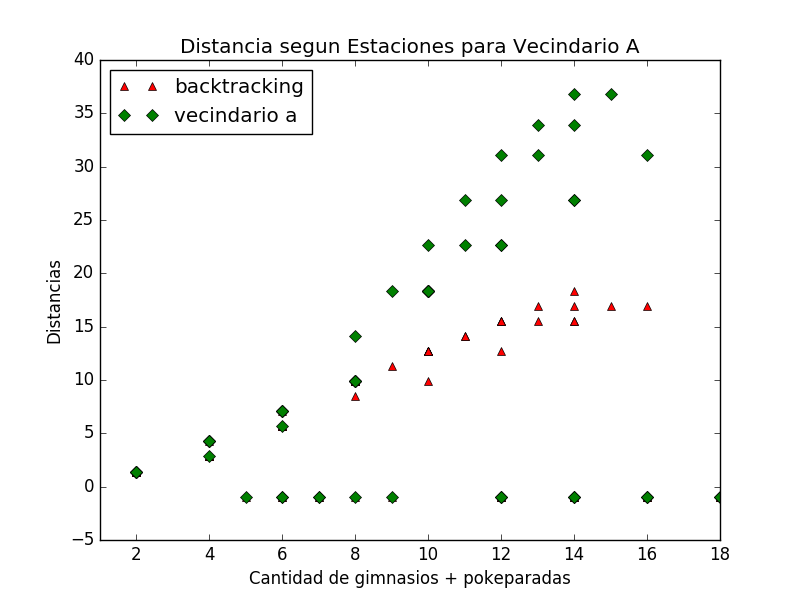
\includegraphics[width=\linewidth]{imagenes/Ej3/Exp2Ej3A.png}
  \caption{Vecindario A}
\endminipage\hfill
\minipage{0.5\textwidth}%
  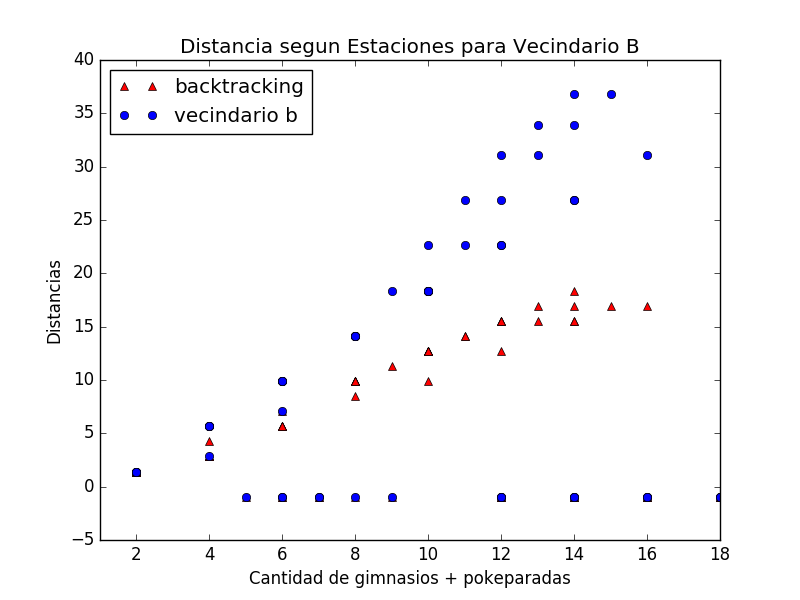
\includegraphics[width=\linewidth]{imagenes/Ej3/Exp2Ej3B.png}
  \caption{Vecindario B}
\endminipage
\end{figure}

\blindtext


\par Para estas instancias, se puede observar que a medida que crece la cantidad de estaciones, crece la brecha entre la solución heurística con búsqueda local, y la solución exacta con backtracking. Esto se debe principalmente a que, a mayor cantidad de estaciones, el campo de soluciones crece. Es decir, mientras que backtracking recorre absolutamente todo el campo de soluciones obteniendo un mínimo global, la búsqueda local a partir de un resultado, recorre únicamente sus vecinos, deteniéndose en los mínimos locales.

\par Además, no esta demás mencionar, que previo a la búsqueda local, se corre un algoritmo greedy y cuya solución devuelta, dada la configuración de nuestras instancias (las cuales aumentan linealmente la cantidad de estaciones, y por cada estación que se agrega se incrementa su ubicación), en la cual se basará la búsqueda local tiende a empeorar a medida que hicimos crecer la cantidad de estaciones (esto es explicado en el \textbf{Ejercicio 2}). Entonces, esto influye directamente en las soluciones encontradas por la búsqueda local, pues debido a que la búsqueda comienza desde una solución la cual puede llegar a diferir de la mejor posible, y que la búsqueda local se detiene en un mínimo local, la mejor solución que encontrará la búsqueda local para cualquier vecindario será peor a la que devuelve el algoritmo exacto, que en nuestro caso, será el mínimo global.

\par Luego dado el vecindario A, se observa que para instancias chicas, las soluciones se asemejan a las exactas pero sus distancias empiezan a diferenciarse a partir 8 estaciones. Mientras que en el vecindario B, desde un primer momento Backtracking encuentra mejores soluciones. Esto nos asegura de que para ciertas instancias, intercambiar pokeparadas hace una mejor búsqueda en el vecindario de soluciones. 

Para poder afirmar nuestra hipótesis, se mostrará a continuación una comparación entre las vecindades y el algoritmo exacto.

  \begin{figure}[H]
      \begin{center}
        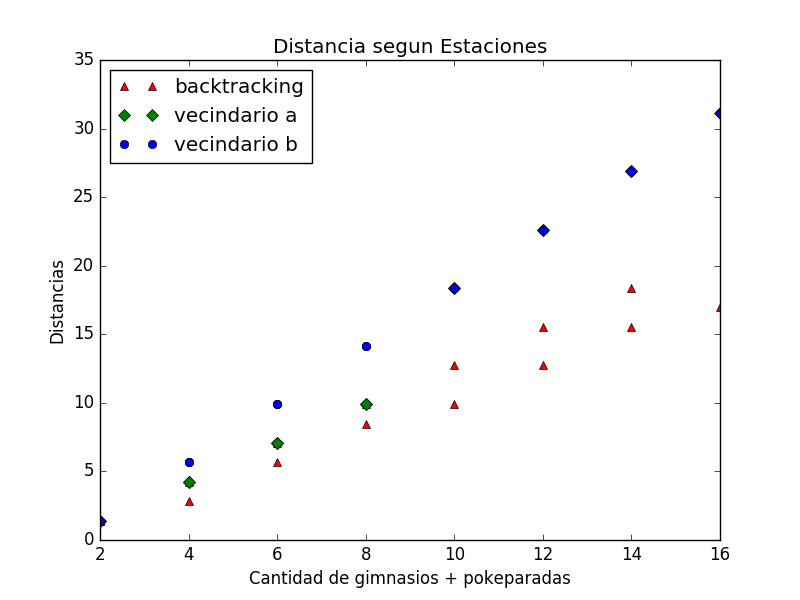
\includegraphics[width=0.7\columnwidth]{imagenes/Ej3/Exp2Ej3TODO.png}
        \caption{Comparación vecindario y backtracking}
      \end{center}
  \end{figure}


Para este caso, se usaron menos instancias para observar el comportamiento de los distintos vecindario en comparación con Backtracking.  Como se puede observar, para instancias chicas las distancias obtenidas por el vecindario A se asemejan a las de backtracking, es decir, a las soluciones exactas. Pero a medida que la cantidad de estaciones crecen, la brecha entre Backtracking y vecindario A crece. Esto mismo no sucede con el vecindario B, donde desde un principio mantiene una brecha creciente con el resultado exacto. Por lo tanto, afirma la hipótesis anteriormente mencionada.

\subsubsection{Experimento 1: Performance} 
            Para experimentar acerca de la performance de los resultados de ambas vecindades, se generaron distintas comparaciones. 

            \begin{itemize}
                \item Por un lado se realizaron comparaciones para la vecindad A, en la cual en cada instancia se intercambian únicamente pokeparadas.
 
                \item Por otro lado, se realizaron comparaciones para la vecindad B, en la cual se intercambian gimnasios (siempre y cuando la solución siga siendo válida).
            \end{itemize}
			
			En ambos casos, se usaron tres tipos de instancias diferentes donde se fijan 4, 5 y 6 gimnasios respectivamente y se aumenta la cantidad de pokeparadas. Por ejemplo, para el primer tipo de instancia se fijan 4 gimnasios y se van agregando pokeparadas.

\blindtext

\begin{figure}[H]
\minipage{0.5\textwidth}
  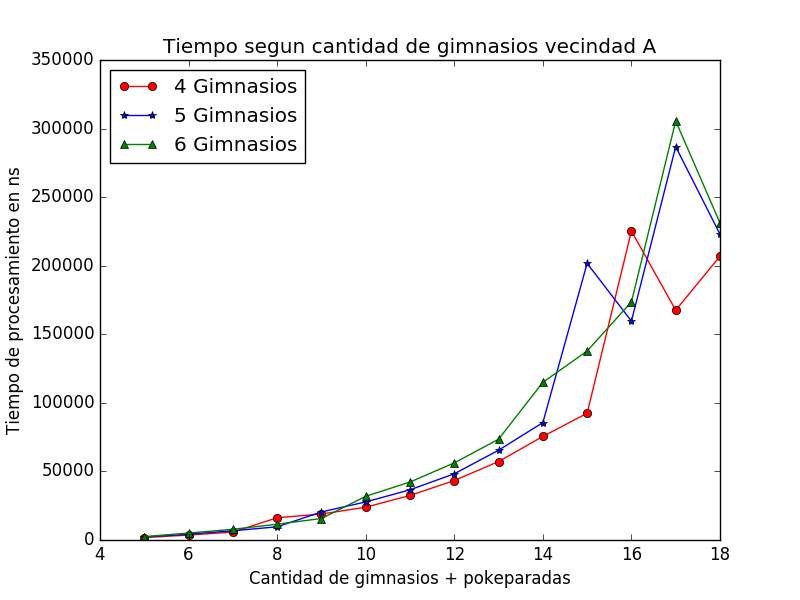
\includegraphics[width=\linewidth]{imagenes/Ej3/Exp1Ej3a.png}
  \caption{Vecindario A}
\endminipage\hfill
\minipage{0.5\textwidth}%
  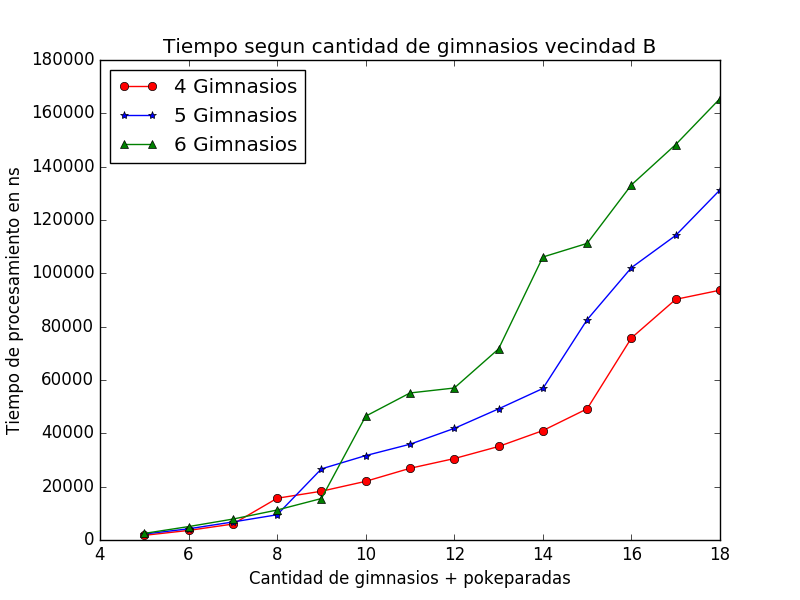
\includegraphics[width=\linewidth]{imagenes/Ej3/Exp1Ej3b.png}
  \caption{Vecindario B}
\endminipage
\end{figure}

\blindtext

Para estas instancias, se puede observar que en ambos casos, a medida que crece la cantidad de estaciones, aumenta el tiempo de procesamiento de manera muy similar.
\par Se puede suponer que para la vecindad A el tiempo de procesamiento debería crecer más rápido que para la vecindad B, debido a que para la vecindad A se pueden intercambiar cualquier par de pokeparadas, mientras que en el vecindario B sólo se pueden intercambiar algunos gimnasios entre sí (además de que para estos experimentos, la cantidad de pokeparadas tiende a ser mucho mayor que la cantidad de gimnasios)
\par Sin embargo, el tiempo de procesamiento es similar ya que para el vecindario B, para cada intercambio de gimnasios se debe chequear que la nueva solución generada sea válida. Y esto implica recorrer cada estación del recorrido, chequeando que para cada gimnasio por el que se pasa, se pase con la cantidad de pokebolas necesarias.


        \subsubsection{Experimento 2}

        En el próximo experimento, comparamos la calidad de solución y el tiempo de corrida de los vecindarios entre sí, y por otro de los vecindarios y el algoritmo greedy, y finalmente los tres juntos. Para esto, se generaron 50 instancias rándom, para cada instancia se corrió el algoritmo 20 veces. Luego se obtuvo un promedio de las 20 corridas hechas para cada instancia (promedio del tiempo de ejecución y de la calidad de la solución).

        \par Para el siguiente experimento queremos probar que realmente, hacer una búsqueda local mejora la solución obtenida del algoritmo heurístico. Esta hipótesis es tomada debido a que, búsqueda local se basa en la solución devuelta por greedy y busca, a partir de ella, encontrar una solución mejor. Por otro lado, queremos ver como se comportan los vecindarios para cualquier instancia, para ver si realmente, dado que el vecindario A tiene más posibilidades de intercambias pokeparadas, esto produce mejores soluciones que el vecindario B, el cuál intercambia gimnasios y tiene menos posibilidades de soluciones válidas.

        \subsubsection{Experimento 2: Calidad de resultados} 

            Para experimentar acerca de la calidad de los resultados, se generaron distintas comparaciones. 

            \begin{itemize}
                \item Por un lado, se compararon los resultados obtenidos ejecutando una búsqueda local haciendo uso del vecindario A, con los obtenidos del vecindario B.
                Dado que el vecindario A da lugar a muchos intercambios posibles, ya que intercambiar dos pokeparadas cualesquiera mantiene una solución válida, mientras que el vecindario B debe descartar varios intercambios de gimnasios ya que algunos pueden dejar un recorrido inválido, nuestra hipótesis fue que la búsqueda local sobre el vecindario A iba a retornar mejores soluciones que la búsqueda local sobre el vecindario B.
 
                \item Por otro lado, se compararon los resultados obtenidos ejecutando una búsqueda local haciendo uso del vecindario A, con los obtenidos a partir del algoritmo greedy (implementado en el Ejercicio 2).
                El objetivo fue poder visualizar que dado una solución obtenida por el algoritmo greedy, ejecutar sobre ésta una búsqueda local, la mejora.
                Elegimos el vecindario A para la búsqueda local ya que es la que más soluciones posibles retorna, debido a la cantidad de intercambios de pokeparadas que se pueden hacer, sobre la cantidad de intercambios de gimnasios que retornan soluciones válidas.
            \end{itemize}

             En ambas comparaciones, se corrió 20 veces el algoritmo sobre cada instancia de 50 obtenidas de forma aleatoria. Luego se sacó un promedio de las 20 distancias devueltas para cada instancia, obteniendo 50 resultados. Y por último, se realizó una comparación de cada resultado en función de la cantidad de estaciones (n+m).
             
             \par A continuación en los siguientes gráficos se pueden observar la calidad de resultados obtenidos en ambas comparaciones.

\blindtext

  \begin{figure}[H]
      \begin{center}
        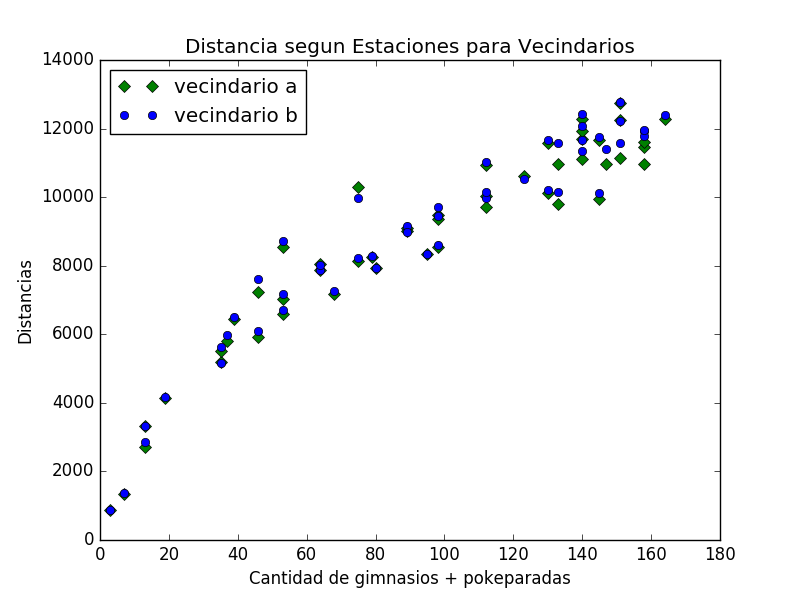
\includegraphics[width=0.7\columnwidth]{imagenes/Ej3/Exp3Ej3ABDistancia.png}
        \caption{Vecindario A vs Vecindario B}
      \end{center}
  \end{figure}

    \begin{figure}[H]
      \begin{center}
        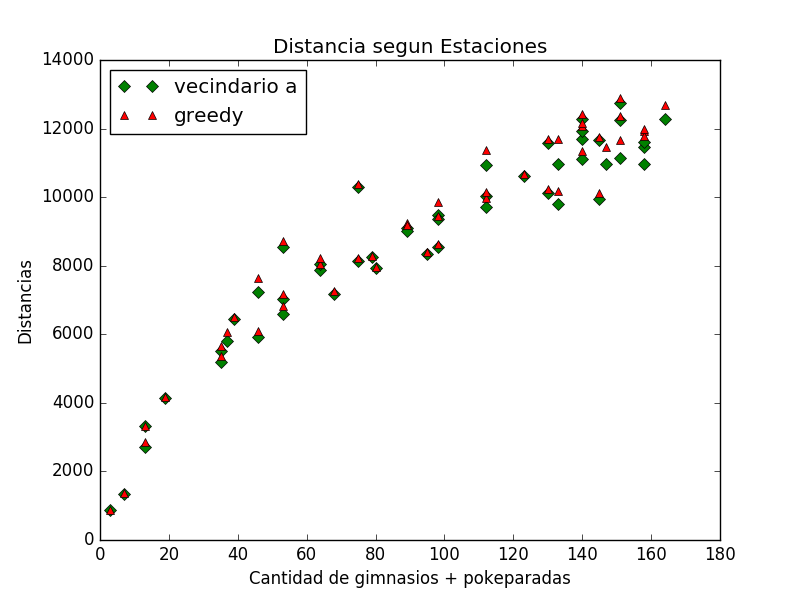
\includegraphics[width=0.7\columnwidth]{imagenes/Ej3/Exp3Ej3AGDistancia.png}
        \caption{Greedy vs Vecindario A}
      \end{center}
  \end{figure}

\blindtext


\par Para el gráfico que compara ambos vecindarios se puede ver que, como suponíamos, las soluciones obtenidas a partir del vecindario A tienden a ser mejores que las soluciones obtenidas a partir del vecindario B.

\par Y de igual manera, para el gráfico que compara la solución obtenida a partir del algoritmo greedy con aplicarle a ésta la búsqueda local usando el vecindario A, se puede ver que, como suponíamos, la búsqueda local mejora las soluciones obtenidas a partir del algoritmo greedy.

\subsubsection{Experimento 2: Performance} 
            Para experimentar acerca de la performance de los resultados de ambas vecindades y del algoritmo greedy sin búsqueda local, se corrió 20 veces cada algoritmo sobre cada instancia de 50 obtenidas de forma aleatoria. Luego se sacó un promedio del tiempo de ejecución (en ns) de las 20 corridas para cada instancia, obteniendo así 50 resultados. Y por último, se realizó una comparación de cada resultado en función de la cantidad de estaciones (n+m).

            \par Nuestra hipótesis fue que en orden de menor a mayor tiempo de procesamiento estaba el algoritmo greedy, el algoritmo con búsqueda local con el Vecindario B, y por último el algoritmo con búsqueda local con el vecindario A.
            \par El algoritmo greedy tenía que ser el más rapido simplemente porque ambas búsquedas locales comienzan ejecutando el algoritmo greedy y luego realizan los intercambios válidos. Al realizar estos intercambios, la diferencia del tiempo de procesamiento aumenta en comparación con el algoritmo greedy.
            \par Y luego, al comparar el tiempo de procesamiento entre ambas vecindades, suponemos que la vecindad A tardará más que la vecindad B, debido a que para la vecindad A se pueden intercambiar cualquier par de pokeparadas, mientras que en el vecindario B sólo se pueden intercambiar algunos gimnasios entre sí (además de que para estos experimentos, la cantidad de pokeparadas tiende a ser mucho mayor que la cantidad de gimnasios).
            Mas allá de que para la búsqueda local con el vecindario B (a diferencia del vecindario A), se deba verificar que para cada intercambio, la solución siga siendo válida (y sino, descartarla), el tiempo sigue siendo mayor debido a que la cantidad de intercambios de pokeparadas es mucho mayor a la cantidad de intercambios de gimnasios que se pueden realizar.

\blindtext

    \begin{figure}[H]
      \begin{center}
        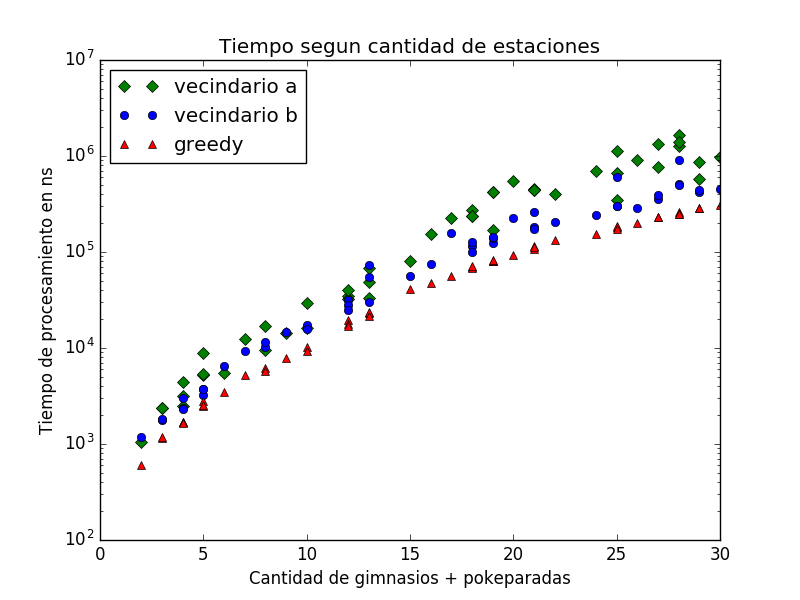
\includegraphics[width=0.7\columnwidth]{imagenes/Ej3/Exp3EJ3TodoTiempo.png}
        \caption{Greedy vs Vecindario A}
      \end{center}
    \end{figure}

\blindtext

En este gráfico se puede observar que el tiempo de procesamiento para cada algoritmo coincide con la hipótesis. La que menos tiempo de procesamiento tiene es la greedy. Luego la búsqueda local con el vecindario B y luego la búsqueda local con el vecindario A.
%\newpage
%\appendix
%\section{Apéndice}\label{sec:codigo}




\end{document}
